\chapter{Data}

Despite the fact that the aim of this work is not to create a database of chants, nor to carry out experiments on data, but rather to create a tool
that researchers can use to conduct trials, we provide a source of data that can be used for the purposes. It is the largest set of digitalized
chants that musicologists regularly use in their research.

Our main source of data is the Cantus database \citep{cantus_db}, one of the databases indexed in the Cantus Index. The database serves as a 
digital archive of chants, each entry containing information about its source, liturgical occasion, mode, and others. Work on the project started
in the late 1980s, and to date, around 500,000 individual chants from approximately 150 manuscripts have been indexed. Each entry is transcribed 
manually and undergoes a thorough examination before publishing \citep{cantus_lacoste}.

We are using a scraped version of the Cantus database released as CantusCorpus \citep{chant21}. Unlike the Cantus database which is continuously being
updated and is therefore unsuitable for computational study, the corpus is versioned, therefore each version always contains the same data. We are using
version 0.2 released in July 2020 which contains 497,071 entries. However, a majority of the data is not suitable for this application, as they do not
contain both melodic and textual data in full, therefore we are only using a subset of size around 13,000. The corpus is available for download in CSV format.

\section{CSV}

CSV is one of the most common formats for tabular data. The abbreviation stands for \emph{comma-separated values}. As the name suggests, the format
uses commas to separate columns (although other separators, such as a semicolon, can be used as well to allow for simpler parsing in case that the data 
frequently contains commas that would otherwise need to be escaped), while the individual rows are separated by a line break. The data is stored as plaintext,
which makes it easily readable. Parsing CSV files becomes more complicated when the data contains column and row separators inside fields; in that case
quotation marks or esape sign has to be used. There exist many well-designed parsers, one such parser is the Python module simply called \emph{csv}\footnote{https://docs.python.org/3/library/csv.html}.
This application uses the module \emph{pandas}\footnote{https://pandas.pydata.org/} to parse CSV files, which in turn uses the \emph{csv} module.

\section{Database fields}
\label{section:db_fields}

Table \ref{table:data_db} represents the data fields in the database.

\begin{longtable}{| p{.25\textwidth} | p{.75\textwidth} |}

 \hline
 Data field & Description \\
 \hline
 id             & automatically generated id in the database \\ \hline
 corpus\_id     & human-readable id identifying the chant in the CantusCorpus \\ \hline
 incipit        & incipit (the first few words) of chant \\ \hline
 cantus\_id     & id identifying the chant in the Cantus Index \\ \hline
 mode           & mode of the chant \\ \hline
 finalis        & the final note of the chant \\ \hline
 differentia    & the melodic ending of psalms \\ \hline
 siglum         & manuscript in which the chant is found \\ \hline
 position       & liturgical role of the chant \\ \hline
 folio          & page of the manuscript where the chant is found \\ \hline
 sequence       & order in which the chant is found in the folio \\ \hline
 marginalia     & clarification about the location of the chant \\ \hline
 cao\_concordances & references to older literature \\ \hline
 feast\_id      & feast of the year during which the chant was sung \\ \hline
 genre\_id      & genre of the chant, e.g. \emph{antiphon}, \emph{responsory} \\ \hline
 office\_id     & office of the day during which the chant was sung, e.g. \emph{Laudes}, \emph{Vespers} \\ \hline
 source\_id     & id of the manuscript in which the chant is found \\ \hline
 melody\_id     & id of melody by which it can be found in the Cantus Index \\ \hline
 drupal\_path   & URL of the chant on the Cantus database website \\ \hline
 full\_text     & full text in a standardized spelling \\ \hline
 full\_text\_manuscript & full text in the manuscript spelling \\ \hline
 volpiano       & transcription of the melody in volpiano format \\ \hline
 notes          & indexing notes \\ \hline
 dataset\_name  & name of the data source to which the chant belongs \\ \hline
 dataset\_idx   & index of the data source to which the chant belongs \\
 \hline

\caption{List of database fields}
\label{table:data_db}
\end{longtable}

\section{User-defined data}
\label{section:data_usr}

The application enables user to upload their own dataset. Table \ref{table:data_usr} specifies the fields in the database. Validation of the
file is not implemented; it is left up to the user to upload a valid file. The meaning of the individual
fields is as described in the previous section unless said otherwise. The value in the column \emph{Required} indicates whether
the column must be present in the file. The value \emph{Nullable} indicates whether a data entry can have \emph{null} or an empty value in the column.
Figure \ref{fig:csv} shows a valid CSV file.

\begin{longtable}{| p{.25\textwidth} | p{.1\textwidth} | p{.1\textwidth} | p{.1\textwidth} | p{.35\textwidth} |}

 \hline
 Column name     & Type & Re\-qui\-red  & Null\-able  & Notes \\
 \hline
 id             & number & no  & yes & the column will be dropped when processing \\ \hline
 corpus\_id     & string & yes & yes &  \\ \hline
 incipit        & string & yes & no  & \\ \hline
 cantus\_id     & string & yes & yes & should be a valid Cantus ID \\ \hline
 mode           & string & yes & yes & \\ \hline
 finalis        & string & yes & yes & \\ \hline
 differentia    & string & yes & yes & \\ \hline
 siglum         & string & yes & no  & \\ \hline
 position       & string & yes & yes & \\ \hline
 folio          & string & yes & yes & \\ \hline
 sequence       & string & yes & yes & \\ \hline
 marginalia     & string & yes & yes & \\ \hline
 cao\_concordances & string & yes & yes & \\ \hline
 feast\_id      & string & yes & yes & \\ \hline
 genre\_id      & string & yes & yes & list of genres is in attachment \ref{attachment:genres} \\ \hline
 office\_id     & string & yes & yes & list of offices is in attachment \ref{attachment:offices} \\ \hline
 source\_id     & string & yes & yes & \\ \hline
 melody\_id     & string & yes & yes & \\ \hline
 drupal\_path   & string & yes & yes & should be a valid URL \\ \hline
 full\_text     & string & yes & no  & \\ \hline
 full\_text\_manuscript & string & yes & yes & \\ \hline
 volpiano       & string & yes & no  & has to be in Volpiano format \\ \hline
 notes          & string & yes & yes & \\ \hline
 dataset\_name  & string & no & yes & the column will be dropped when processing \\ \hline
 dataset\_idx   & number & no & yes & the column will be dropped when processing \\
 \hline

\caption{Fields in the user-uploaded CSV}
\label{table:data_usr}
\end{longtable}

\begin{figure}[h]
\centering
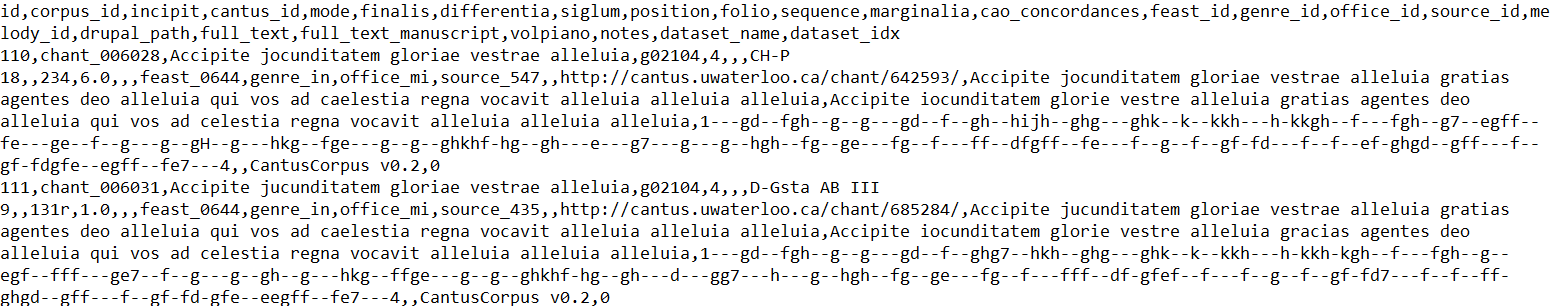
\includegraphics[scale=0.4]{data_csv-example}
\caption{Example of a valid CSV file}
\label{fig:csv}
\end{figure}

\section{Melody encoding}

The melodies in the volpiano fields are encoded as strings of alphanumeric characters and dashes. These can be rendered as musical notation using
the Volpiano font. Each character represents either a pitch, empty space, or other musical characters, such as a clef.

Volpiano was developed as a research tool optimized for databases and word processors. There are strict rules concerning the transcription, which leads
to all Volpiano-encoded melodies having a standardized format. For example, the Volpiano protocol dictates that each transcription begins with
a treble clef followed by three spaces, that words are separated by three spaces and syllables by two, and others.
\footnote{\url{https://cantus.uwaterloo.ca/sites/default/files/documents/2.\%20Volpiano\%20Protocols.pdf}} Figure \ref{fig:volpiano} shows an example
of an encoded melody along with its rendering.

\begin{figure}[h!]
\centering
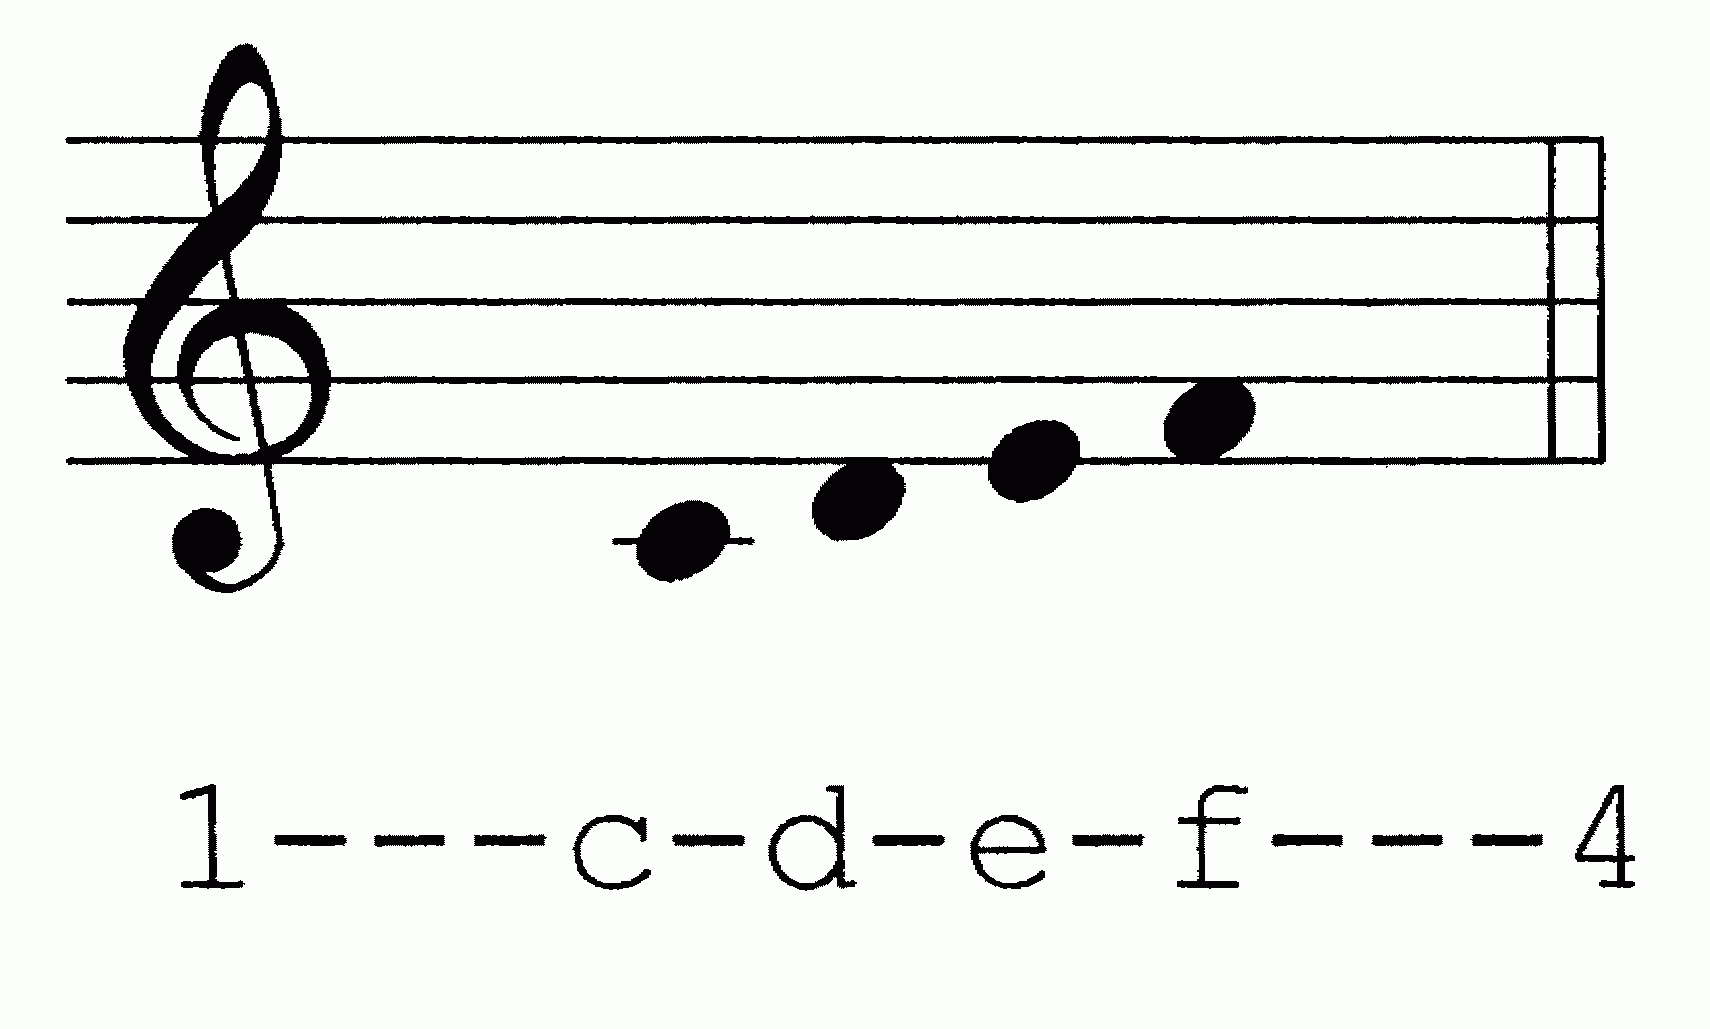
\includegraphics[scale=0.1]{volpiano}
\caption{Example of volpiano as stored in the database and how it is rendered as musical notation. \cite[Figure~2]{cantus_lacoste}}
\label{fig:volpiano}
\end{figure}

\section{Data statistics}

As mentioned earlier, not all of the almost 500,000 entries in the CantusCorpus can be aligned.
As one of the application's main features is melody alignment, it is necessary that we only use those data points whose \emph{volpiano} field is
not empty. Moreover, some visualizations compare text length to melody length, therefore we require the data points to have both. Additionally, 
text and melody should be able to be aligned, i.e. they contain the same number of words and syllables.

After removing the data that does not adhere to the conditions, we are left with 13,397 usable data points.

In the rest of this section, we outline the basic statistics about the data. We concentrate in particular on the length of the chants'
melodies and lyrics, as these characteristics tend to differ among genres. This information is not necessary for the understanding of
the thesis. However, it shows the diversity of the chant repertoire and allows us to visualize the amount of information contained
in the data.

The dataset contains entries of 37 different genres. 14 of them are associated with more than 100 entries. Figure \ref{fig:genre-counts}
shows their distribution. The following statistics are done on the subset of all data whose entries belong to one of these genres.
The list of genres corresponding to each genre ID is in attachment \ref{attachment:genres}.

\begin{figure}[h!]
\centering
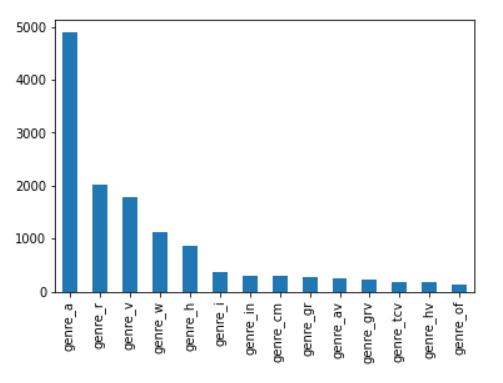
\includegraphics{data_genre-counts}
\caption{Distribution of genres in the dataset.}
\label{fig:genre-counts}
\end{figure}

Table \ref{table:genres} shows the mean and the standard deviation of text and melody length by genres. Text length is defined as the number of words
(strings separated by spaces). Melody length is defined as the number of non-gap characters (\verb|-|) in the Volpiano encoding.

\begin{longtable}{| p{.2\textwidth} | p{.15\textwidth} | p{.15\textwidth} | p{.15\textwidth} | p{.15\textwidth} |}

\hline
Genre ID & mean text length & standard deviation of text length & mean melody length & standard deviation of melody length \\
\hline
genre\_a & 9.9 & 8.0 & 38.3 & 38.8 \\
genre\_av & 7.4 & 2.9 & 22.5 & 13.0 \\
genre\_cm & 14.6 & 7.1 & 82.6 & 36.0\\
genre\_gr & 9.2 & 4.5 & 99.1 & 54.4 \\
genre\_grv & 10.9 & 3.7 & 141.8 & 44.7 \\
genre\_h & 5.2 & 5.5 & 29.0 & 22. 4 \\
genre\_hv & 12.8 & 5.2 & 50.7 & 21.9 \\
genre\_i & 4.7 & 3.5 & 28.0 & 24.6 \\
genre\_in & 16.6 & 7.5 & 99.4 & 41.9 \\
genre\_of & 11.9 & 9.3 & 103.3 & 77.9 \\
genre\_r & 4.9 & 5.5 & 28.9 & 45.3 \\
genre\_tcv & 10.7 & 3.3 & 102.9 & 28.2 \\
genre\_v & 7.0 & 4.6 & 36.8 & 24.8 \\
genre\_w & 3.3 & 1.6 & 11.0 & 6.2 \\
\hline

\caption{Mean text and melody length and standard deviation of chants grouped by genres.}
\label{table:genres}
\end{longtable}

Figure \ref{fig:genres-scatter} shows the comparison of text length to melody length for the individual genres.

\begin{figure}[h!]
\centering
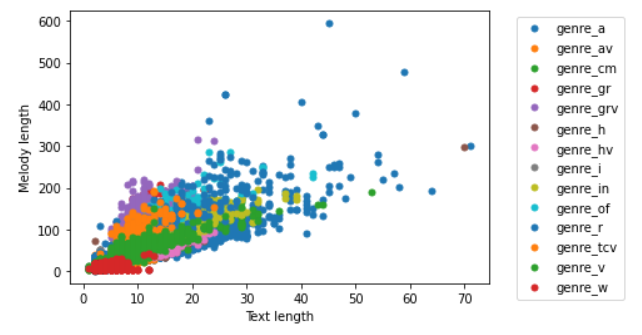
\includegraphics{data_genres-scatter}
\caption{Approximate visual comparison of text length and melody length for each genre.}
\label{fig:genres-scatter}
\end{figure}

Now, we will show the same statistics for chants divided by their offices. First, Figure \ref{fig:office-counts} shows the distribution of the offices
among the dataset. The list of office names corresponding to each office ID can be found in attachment \ref{attachment:offices}.

\begin{figure}[h!]
\centering
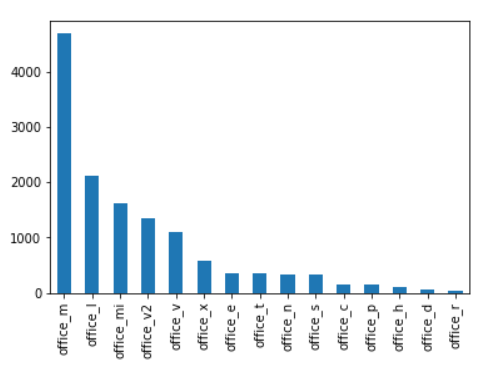
\includegraphics{data_office-counts}
\caption{Distribution of offices in the dataset.}
\label{fig:office-counts}
\end{figure}

Table \ref{table:offices} shows the mean and the standard deviation of text and melody length of the datasets.

\begin{longtable}{| p{.2\textwidth} | p{.15\textwidth} | p{.15\textwidth} | p{.15\textwidth} | p{.15\textwidth} |}

\hline
Office ID & mean text length & standard deviation of text length & mean melody length & standard deviation of melody length \\
\hline
office\_c & 9.8 & 8.3 & 38.7 & 37.5 \\
office\_d & 5.0 & 2.6 & 19.9 & 20.2 \\
office\_e & 14.0 & 8.8 & 50.0 & 33.7 \\
office\_h & 14.2 & 7.3 & 65.8 & 37.4 \\
office\_l & 8.3 & 6.4 & 30.4 & 25.0 \\
office\_m & 6.9 & 10.0 & 33.8 & 43.7 \\
office\_mi & 13.1 & 10.3 & 102.8 & 54.8 \\
office\_n & 5.4 & 4.6 & 19.8 & 16.9 \\
office\_p & 4.9 & 4.5 & 18.4 & 20.4 \\
office\_r & 9.3 & 6.1 & 35.44 & 34.4 \\
office\_s & 4.9 & 3.8 & 17.9 & 15.5 \\
office\_t & 5.3 & 3.8 & 19.0 & 15.9 \\
office\_v & 6.8 & 7.7 & 29.0 & 36.0 \\
office\_v2 & 6.8 & 7.1 & 26.4 & 31.0 \\
office\_x & 13.1 & 10.8 & 61.0 & 52.3 \\
\hline

\caption{Mean text and melody length and standard deviation of chants grouped by office.}
\label{table:offices}
\end{longtable}

Finally, Figure \ref{fig:offices-scatter} compares lengths text and melody of chants divided by genres.

\begin{figure}[h!]
\centering
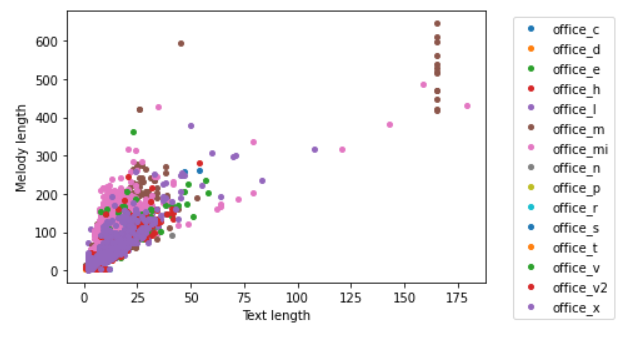
\includegraphics{data_offices-scatter}
\caption{Approximate visual comparison of text length and melody length for each office. From this visualization it is already clear that there is a group
of chants from the morning prayer that merits further investigation.}
\label{fig:offices-scatter}
\end{figure}
